\chapter{Исследовательская часть}

В данном разделе будет приведен пример работы программы, а также проведен сравнительный анализ алгоритмов при различных ситуациях на основе полученных данных.

\section{Технические характеристики}

Технические характеристики устройства, на котором выполнялся эксперимент представлены далее:

\begin{enumerate}[label=\arabic*)]
	\item операционная система --- Ubuntu 22.04.3~\cite{ubuntu} Linux x86\_64;
	\item память --- 16 Гб;
	\item процессор --- Intel® Core™ i5-1135G7 @ 2.40 ГГц.
\end{enumerate}

При эксперименте ноутбук не был включен в сеть электропитания.

\section{Демонстрация работы программы}

На рисунке \ref{fig:example} представлен результат работы программы для обоих рассматриваемых алгоритмов.
\clearpage

\begin{figure}[h!]
	\centering
	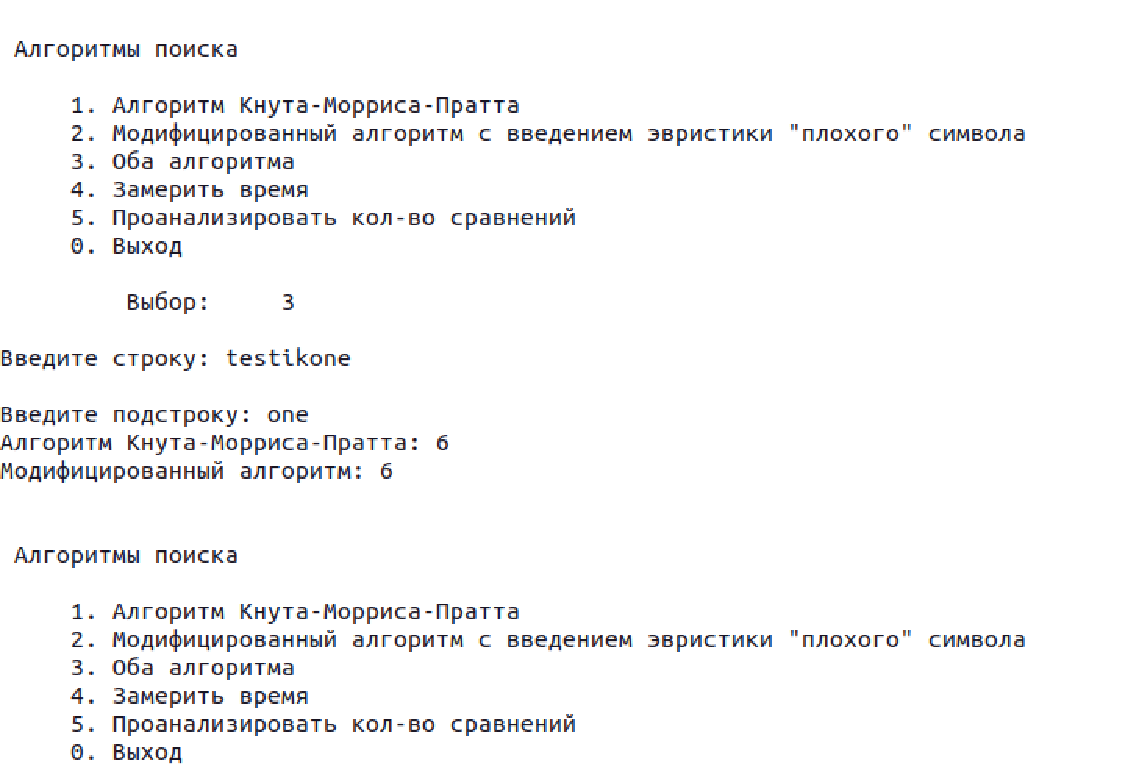
\includegraphics[width=0.9\linewidth]{img/example}
	\caption{Пример работы программы}
	\label{fig:example}
\end{figure}


\section{Время выполнения алгоритмов}

Как было сказано выше, используется функция замера процессорного времени  \textit{process\_time(...)} из библиотеки \textit{time} на \textit{Python}. 
Функция возвращает процессорное время типа float в секундах.

Функция используется дважды: перед началом выполнения алгоритма и после завершения, затем из конечного времени вычитается начальное, чтобы получить результат.

Замеры проводились при длине строки в 30 символов, длине подстроки в 3 символа и разном расположении подстроки в строке.
Для каждого расположения время находилось 250 раз и затем усреднялось.

Результаты замеров приведены на рисунке \ref{fig:graph_time} в графическом виде.

\begin{figure}[h!]
	\centering
	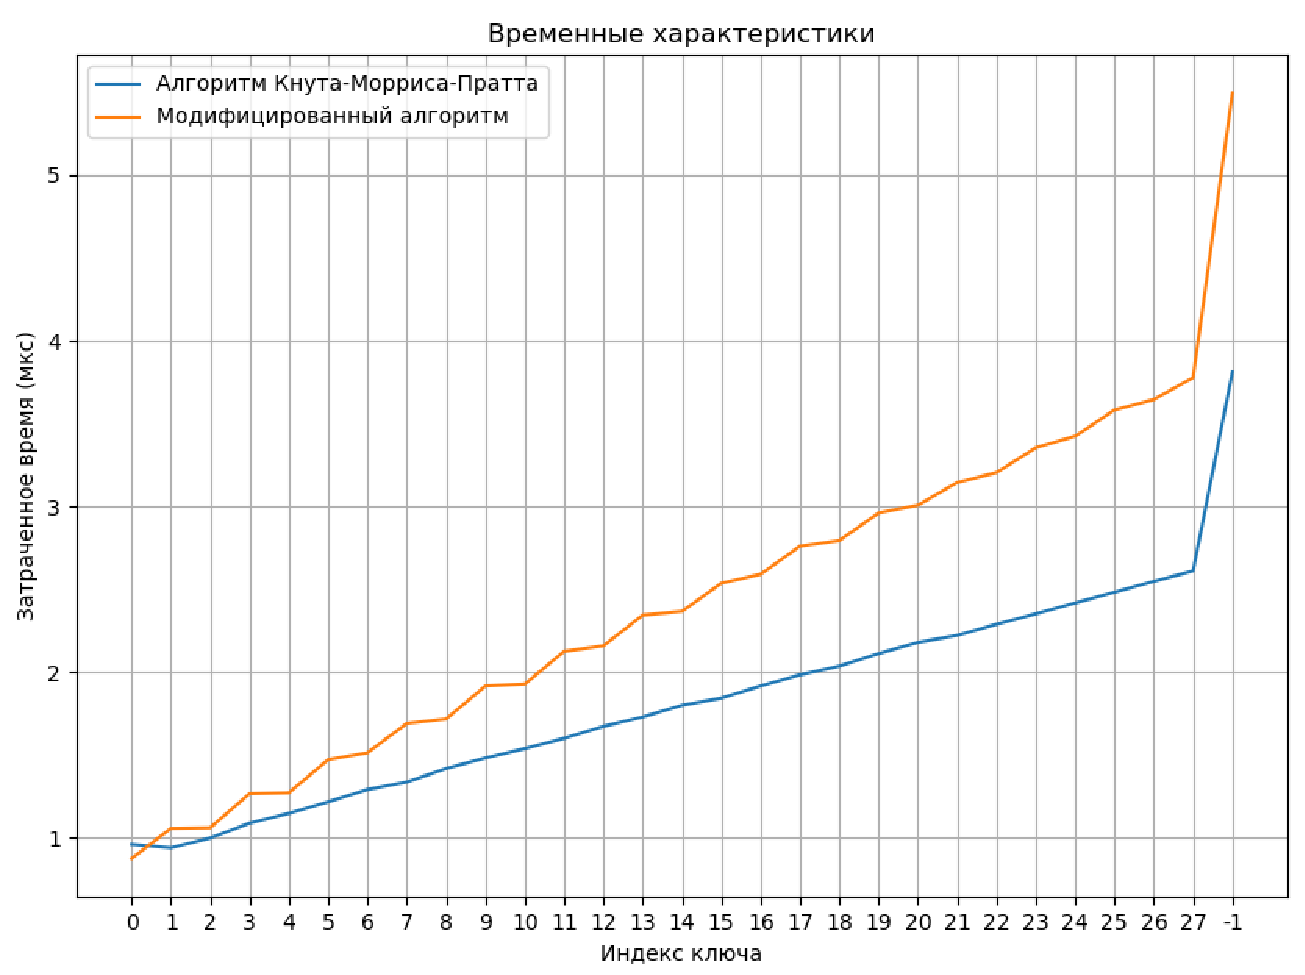
\includegraphics[width=0.8\linewidth]{img/time}
	\caption{Сравнение по времени алгоритмов}
	\label{fig:graph_time}
\end{figure}

\section[Количество сравнений при работе алгоритмов]{Количество сравнений при работе \\алгоритмов}

Для каждого алгоритма был проведен анализ по количеству сравнений для нахождения подстроки в строке.
Строка бралась длиной 33 символа, подстрока длиной 3 символа, расположение --- разное.

На рисунке \ref{fig:graph_kmp} представлена гистограмма с количеством сравнений для поиска алгоритмом Кнута-Морриса-Пратта, на рисунке \ref{fig:graph_bm} --- его модификацией с использованием эвристики <<плохого>> символ.

\begin{figure}[h!]
	\centering
	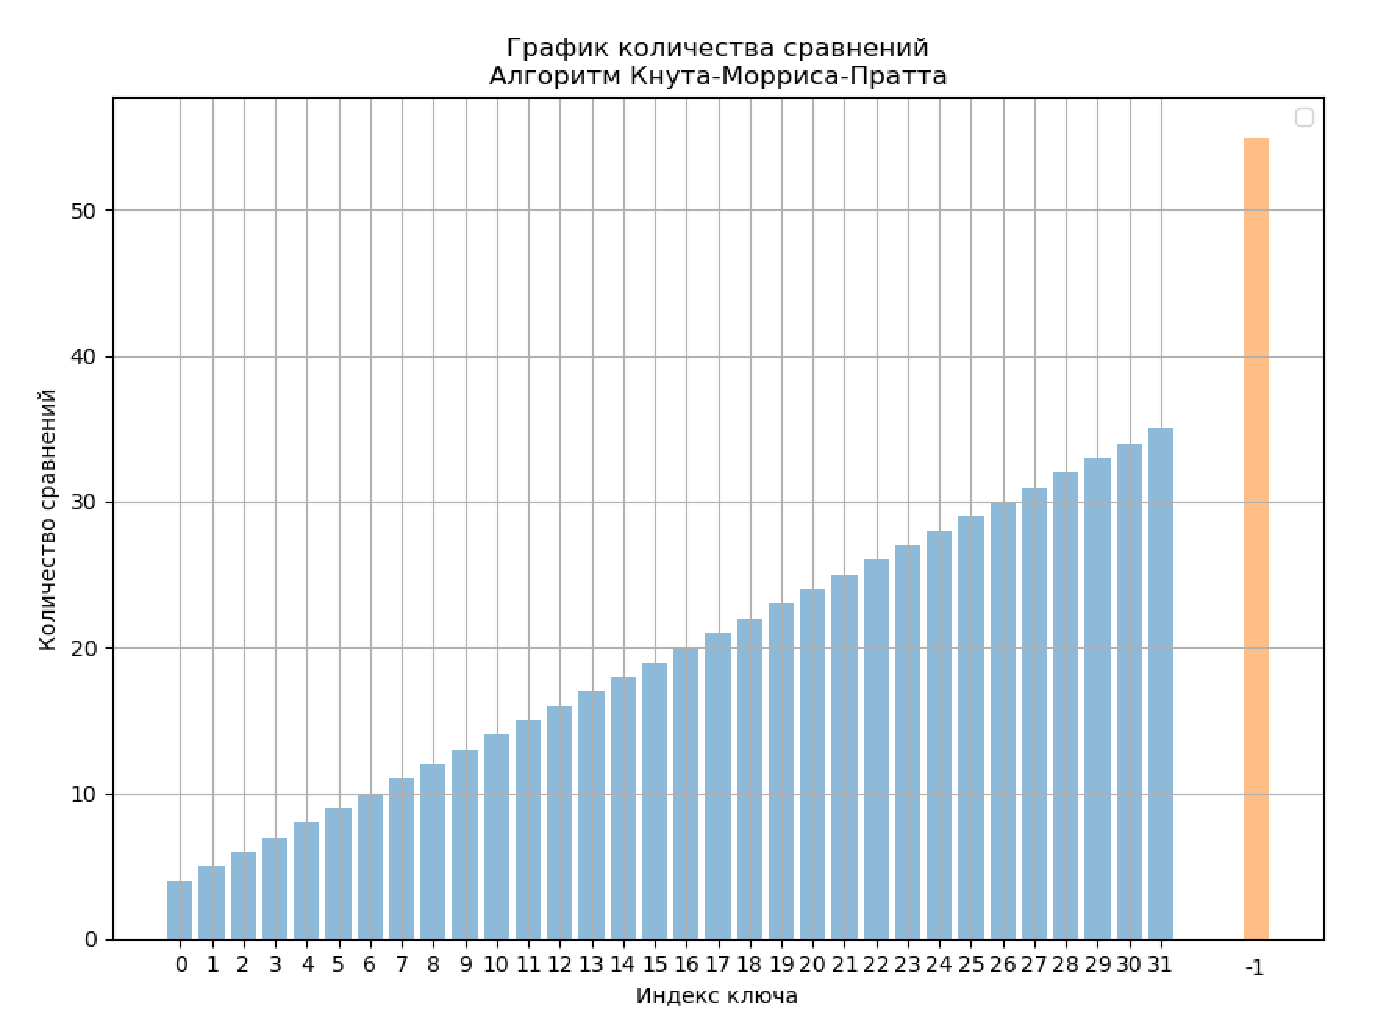
\includegraphics[width=0.9\linewidth]{img/kmp_c}
	\caption{Количество сравнений для алгоритма Кнута-Морриса-Пратта}
	\label{fig:graph_kmp}
\end{figure}

\begin{figure}[h!]
	\centering
	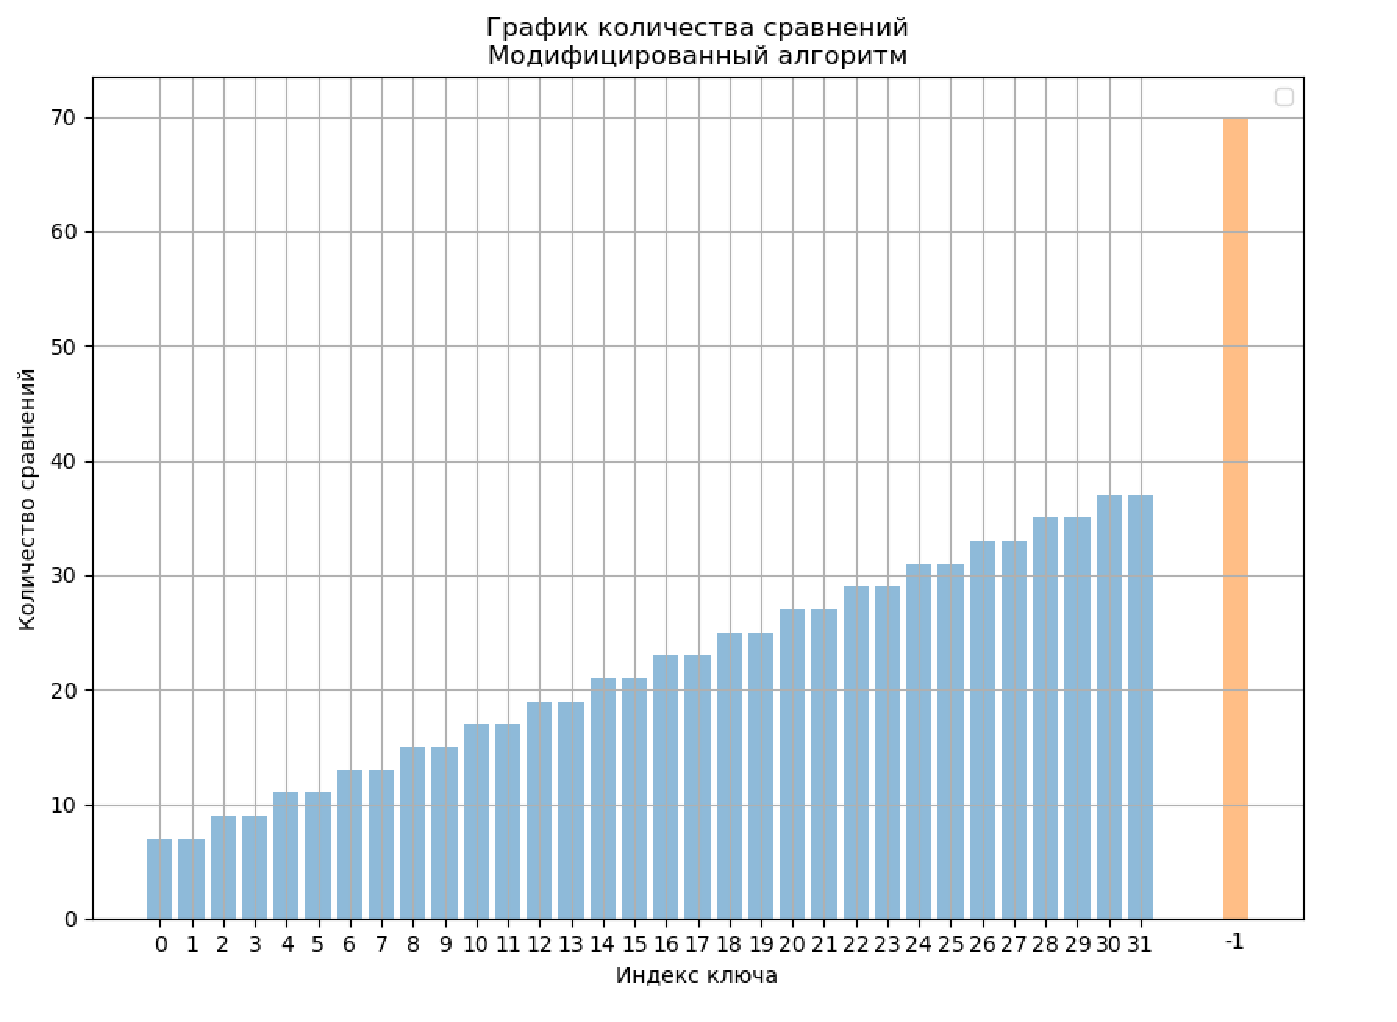
\includegraphics[width=0.9\linewidth]{img/bm_c}
	\caption{Количество сравнений для модифицированного алгоритма}
	\label{fig:graph_bm}
\end{figure}

\clearpage


\section{Вывод}

В результате эксперимента было получено, что худший случай для этих алгоритмов --- отсутствие подстроки в строке.
Реализация алгоритма Кнута-Морриса-Прата работает примерно в 1.5 раза быстрее реализации модифицированного алгоритма, но при этом использует примерно в 2 раза больше операций сравнения.
